%Template created by Maytee Cruz-Aponte for MTBI 2011
\documentclass[size=custom,width=48 in,height=42 in, landscape]{sciposter}
\usepackage{amsmath}
\usepackage{amssymb}
\usepackage{gensymb}
\usepackage{siunitx}
\usepackage{array}
\usepackage{comment}
\usepackage{multicol}
\usepackage[english]{babel}
\usepackage[pdftex]{graphicx}
\usepackage[round,numbers,sort&compress]{natbib}
\usepackage{tikz}
\usepackage{booktabs}
\usepackage[utf8]{inputenc}
\usepackage{tabularx}
\usepackage{color} 
\usepackage[many]{tcolorbox}
\usepackage{lmodern} 
\usepackage{mathtools}
\usepackage{bm}
%\usepackage[listings]{tcolorbox}
\usepackage[left=1cm,right=4cm,bottom=0cm,top=1.5cm]{geometry} 
\tcbuselibrary{listings,theorems, skins, raster}
\usetikzlibrary{shapes.geometric, arrows}
\tikzstyle{rect} = [rectangle, rounded corners, minimum width=2cm, minimum height=1cm,text centered, draw=black,opacity = 0.5]
\tikzstyle{squ} = [rectangle, rounded corners, minimum width=2cm, minimum height=2cm, text centered, draw=black]
\tikzstyle{arrow} = [thick,->,>=stealth]
\renewcommand{\bibnumfmt}[1]{#1.}
% Footnotes
\long\def\symbolfootnote[#1]#2{\begingroup%
\def\thefootnote{\fnsymbol{footnote}}\footnote[#1]{#2}\endgroup}
\bibliographystyle{plainnat}
\bibpunct{(}{)}{;}{a}{,}{,}
\usepackage{booktabs} % Top and bottom rules for tables
\usepackage{enumitem} % Used to reduce itemize/enumerate spacing
\renewcommand{\papertype}{custom} \renewcommand{\fontpointsize}{10pt}
%\setlength{\paperwidth}{91.44cm} \setlength{\paperheight}{91.44cm}
\usepackage{authblk}
\usepackage{transparent}
\usepackage{eso-pic}
\newcommand\BackgroundPic{%
\hspace{-1 cm}
\put(0,0){%
\parbox[b][\paperheight]{\paperwidth}{%
{\transparent{0.2} \includegraphics[width=48 in,height=42 in]{pic2.jpg}}%
\vfill
}}}

\makeatletter
\renewcommand\AB@affilsepx{ , \protect\Affilfont}
\makeatother

\title{\huge{An Age Structured Model of the Impact of Buffelgrass on Saguaro Cacti and their Nurse Trees}}

\renewcommand\Authfont{\fontsize{35}{0}\selectfont}
\renewcommand\Affilfont{\fontsize{30}{0}\itshape}


\author[1]{Lucero Rodriguez-Rodriguez}
\author[2]{Erin Stafford}
\author[3]{Anna Williams}
\author[4]{Brian Wright}
\affil[1]{University of Texas Rio Grande Valley}
\affil[2]{Tulane University}
\affil[3]{University of Texas at Austin}
\affil[4]{University of Redlands}
%\email{\large{corresponding author email}}  % shows author email address below institute

 
\leftlogo[.75]{ASU.pdf} % defines logo to left of title (with scale factor)
\rightlogo[.75]{MTBILogo.png}   %same but on right
\definecolor{BoxCol}{rgb}{.6431,0,.2745} %white % Defines the color used for content box headers
\definecolor{SectionCol}{rgb}{1,1,1}
\newcommand{\compresslist}{ % Define a command to reduce spacing within itemize/enumerate environments, this is used right after \begin{itemize} or \begin{enumerate}
\setlength{\itemsep}{1pt}
\setlength{\parskip}{0pt}
\setlength{\parsep}{0pt}
}
%%% Begin of Document

\begin{document}
\AddToShipoutPicture*{\BackgroundPic}
\usetikzlibrary{patterns}
%define conference poster is presented at (appears as footer)
\conference{MTBI@ASU 2011}
\maketitle
\vspace{-2cm}
\section{Abstract}
The saguaro cactus (Carnegiea gigantea), a keystone species in the Sonoran Desert, has faced population decline in recent years. The immediate threat to the saguaro cactus is the increase in wildfires fueled by the invasive species buffelgrass (Pennisetum ciliare). The increasing rate of wildfires could result in the collapse of the Sonoran Desert ecosystem. A stage structured model is used to capture interactions between saguaro cacti (juvenile and adults), their nurse trees, and buffelgrass. The introduction of buffelgrass to the model demonstrates its influence on the natural life cycles of the saguaro and nurse tree populations. This model consists of a system of non--linear ordinary differential equations which considers commensalism between juvenile saguaros, their nurse trees, and the eventual competition between adults and nurse trees. Both qualitative analysis of the equilibria of the system as well as a numerical analysis of the sensitivity of key parameters are done. In the interest of preserving the saguaro cactus population, this model will provide insight into the effectiveness of current mitigation strategies. 

%%% Begin of Multicols-Enviroment
\begin{multicols}{3}
\section{Introduction}
Since the saguaro cactus serves as a habitat and food source for many other species in the region, changes in the saguaro cactus population indicates the health of the  ecosystem. The cactus is important for the tourism industry and has cultural significance to the Papago and Pima nations. In 1989, buffelgrass was introduced to Saguaro National Park. Buffelgrass is an invasive species able to grow close in proximity to other plants. As a fire-adapted plant, buffelgrass is able to survive fires and quickly regrow. Therefore, buffelgrass acts as a prevalent fuel for fires, quickly burning native plants like saguaros and nurse trees and replacing them within weeks. \\

\vspace{-1cm}
\begin{figure}
\centering
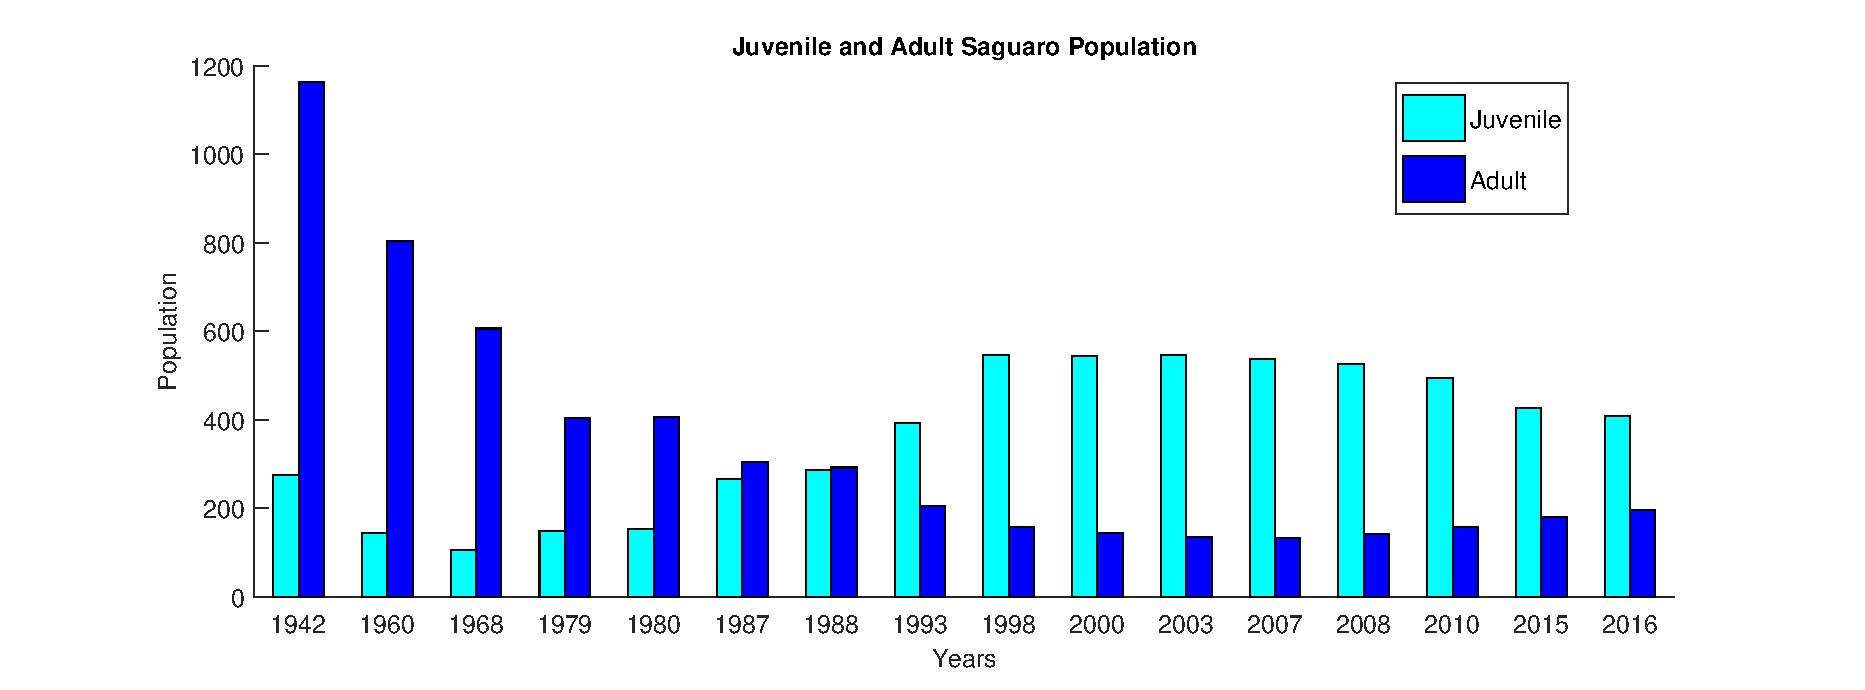
\includegraphics[trim={1.5cm 0 3cm 0},clip,scale = .8]{sagpop.eps}
\tiny{\caption{Population data collected for the saguaro population from 1942 to 2016.}}
\end{figure}
\vspace{-1.5cm}
\section{The Model Assumptions}
\small{
\begin{itemize}
\itemsep0em 
\item Juvenile saguaros are assumed to be cacti in the age range of 1 to 35.
\item The natural life span of all adult saguaros is 175 years, which is the average lifespan.
\item Nurse trees are not able to out compete adult saguaros for resources
\item Juvenile saguaros compete over space with adult saguaros.
\item Nurse trees increase the available space for juvenile saguaros
\item Competition or commensalism between buffelgrass and other species is minimal and is neglected.
\item Buffelgrass harms saguaros and nurse trees through the propagation of wildfire.
\item Since buffelgrass is a fire-adapted species, it is not harmed by wildfire and regrows quickly after fires.
\end{itemize}}

\section{The Model}
The model is formulated using the dynamics between the adult and juvenile saguaro cacti, their nurse trees, and buffelgrass. The interactions considered are given by the equations below.
%\begin{subequations}

\boldmath
\begin{eqnarray*}
&\displaystyle\frac{dS_j}{dt}&= rS_a\cdot \text{max}\left\lbrace0,\left(1-\displaystyle\frac{\epsilon S_j + S_a}{k_1+b T}\right) \right\rbrace - \gamma S_j - \mu_j S_j - \theta_j B S_j\\
&\displaystyle\frac{dS_a}{dt}& = \gamma S_j -\displaystyle\frac{\alpha_1}{k_2}S_a T - \mu_a S_a - \theta_a B S_a\\
&\displaystyle\frac{dS_T}{dt}& = \phi T\left(1 - \displaystyle\frac{T + \sigma S_a}{k_2}\right) - \theta_T B T\\
&\displaystyle\frac{dB}{dt}& = \omega B \left(1-\displaystyle\frac{B}{k_3}\right) - \mu_B B\\
\end{eqnarray*}

\vspace{-1cm}
\section{Parameters}
\begin{figure}
\centering

\setlength{\arrayrulewidth}{.3mm}
\setlength{\tabcolsep}{20pt}
\renewcommand{\arraystretch}{1.5}


{\tiny \centering \hspace{-.8cm}\begin{tabular}{ |p{2cm}|p{6.5cm}| p{2cm}| p{6.5cm}|}

\hline
\multicolumn{4}{|c|}{Parameters} \\
\hline
Parameter& Description & Parameter & Description\\
\hline
$r$ & Germination rate & $k_1$& Adult saguaro carrying capacity\\
\hline

$\epsilon$ & Converts juveniles to adults & $b$ & Average juveniles under nurse tree\\
\hline

$\gamma$& Maturation rate & $\mu_j$ & Juvenile death rate\\
\hline

$\alpha_1$& Saguaro death rate by competition & $k_2$ & Carrying capacity of adults and trees\\
\hline

$\mu_a$ & Adult death rate & $\phi$ & Growth tree population\\
\hline
$\rho$ & Tree competition death rate & $\sigma$ & Proportion carrying capacity\\
\hline
$\theta_j$ & Grass fire frequency effect-juvenile& $\theta_a$ & Grass fire frequency effect-adult\\
\hline
$\theta_t$ &Grass fire frequency effect-tree & $\omega$ & Grass growth rate\\
\hline
$\mu_b$ & grass harvesting & $k_3$ & Carrying capacity of grass\\
\hline
 \hline 
\end{tabular}}

\end{figure}
\columnbreak

\vspace{-1.5cm}
\section{Results of the Equilibria Analysis}
In order to maintain a stable population equilibrium, several requirements were found. The expected number of adult saguaro cacti produced by one adult saguaro must be greater than one to for population maintenance among the cacti. Without nurse trees, this conditions is given by,
$$R_{d1} = \displaystyle\frac{\gamma}{\gamma+\mu_j} \cdot\displaystyle\frac{r}{\mu_a} > 1$$
With nurse trees, this conditions is given by,
$$R_{d2} = \displaystyle\frac{r}{\mu_a+\alpha}\cdot\frac{\gamma}{\gamma + \mu_j} > 1$$
\begin{center}
\setlength{\arrayrulewidth}{.5mm}
\setlength{\tabcolsep}{18pt}
\renewcommand{\arraystretch}{1.5}

{\tiny\hspace{-.5cm}\begin{tabular}{ |p{7cm}|p{7cm}|p{7cm}|}
\hline
Equilibrium & Existence & Stability \\
\hline
$E_1= (0,0,0,0)$ & always & unstable\\

$E_2= (0,0,T_2^*,0)$ & always & $R_{d4} < 1$ and $\omega<\mu_b$ \\

$E_3= (S_{j3}^*, S_{a3}^*, 0,0)$ & $R_{d3} > 1$ & $\displaystyle\frac {\phi}{\rho}<\displaystyle\frac{k_1}{1+\tilde{E}}\left(1-\displaystyle\frac{1}{R_{d3}}\right) $ \\

$E_4= (S_{j4}^*, S_{a4}^*, T_4^*, 0)$ & If, with $\tilde{S_a^*} < \displaystyle\frac{\phi}{\rho}, R_{d3} > 1$& Stable(numerical)\\

$E_5= (0,0,0,B^*)$ & always & unstable\\

$E_6= (0,0,T_2^*, B^*)$ & always & $R_{d2} < 1$ and $\omega<\mu_b$ \\

$E_7= (S_{j3}^*, S_{a3}^*, 0, B^*)$ & $ R_{d1} > 1$ & $\displaystyle\frac {\phi}{\rho}<\displaystyle\frac{k_1}{1+\tilde{E}}\left(1-\displaystyle\frac{1}{R_{d1}}\right) $ \\

$E_8=(S_{j4}^*,S_{a4}^*,T_4^*,B^*)$ & If, with $\tilde{S_a^*} < \frac{\phi}{\rho}$,$R_{d4} > 1$ and $\displaystyle\frac{\phi}{\rho} > \displaystyle\frac{k_1}{1+\tilde{E}}\left(1-\frac{1}{R_{d1}}\right)$ then there is at least one coexistence equilibrium. & Stable (numerical) \\

\hline

\end{tabular}}
\end{center}
\section{Results of the Numerical Analysis}

Numerical simulations  and a local sensitivity analysis were performed. From the numerical simulations, it can be seen that with the current wildfire frequency, the saguaro and nurse tree populations are able to coexist with buffelgrass.\\

\vspace{-1cm}
\begin{figure}
\centering
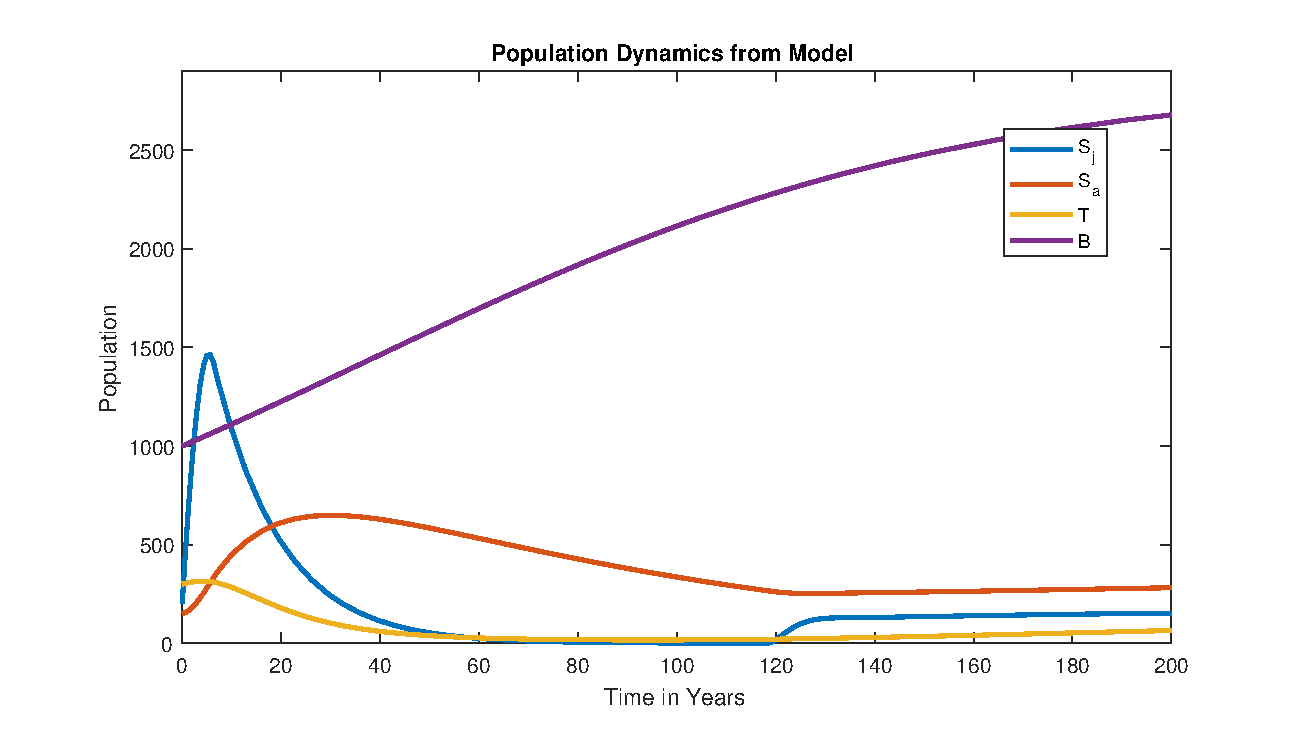
\includegraphics[scale = 0.7]{buffelModel.eps}
\tiny{\caption{The population dynamics given in the figure use the baseline parameter values and show that no population approaches extinction. Although the tree population appears to die out, this does not occur at any point in the time span.}}
\end{figure}

However, if the wildfire frequency increases, saguaros and nurse trees would be put at risk.\\

\begin{figure}
\vspace{-1cm}
\centering
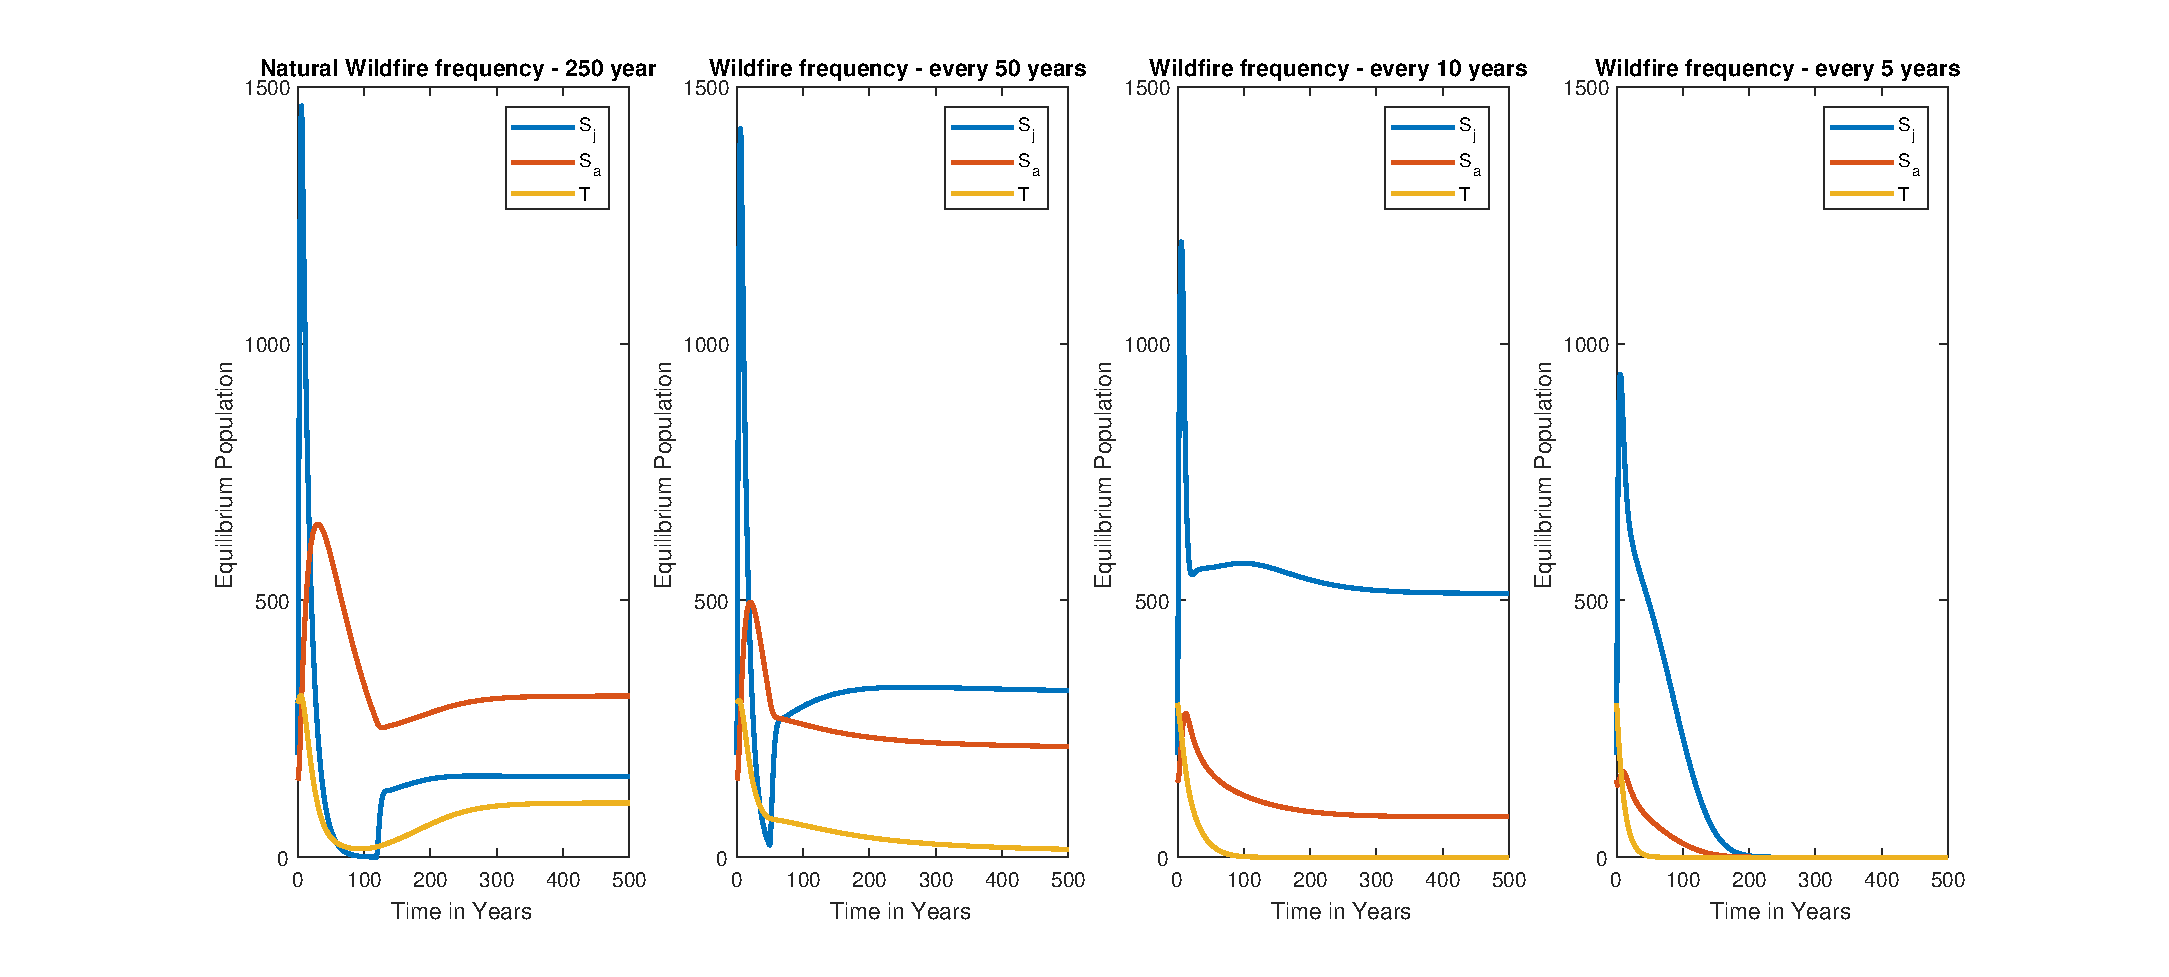
\includegraphics[scale = 0.6]{IncreasingWildfireFrequancy.eps}
\tiny{\caption{This figure show the population dynamic of saguaros and nurse trees changing in response to increased wildfire frequency.}}
\end{figure}

The natural wildfire frequency of 250 years allows coexistence of all species. However, if the frequency is increased to 10 years, nurse trees die out, and if it is further increased to 5 years, saguaros also die out. Since the frequency of wildfires is currently increasing, this means saguaros and nurse trees are at a greater risk.\\
\section{Cont. Numerical Results}
The best way to reduce this risk according the both the simulation and sensitivity analysis is to reduce the buffelgrass population by decreasing $\omega$, the growth rate of the buffelgrass population, and increasing $\mu_B$, the harvesting rate affecting the buffelgrass population.\\

\vspace{-1cm}
\begin{figure}
\hspace{1 cm}
\centering
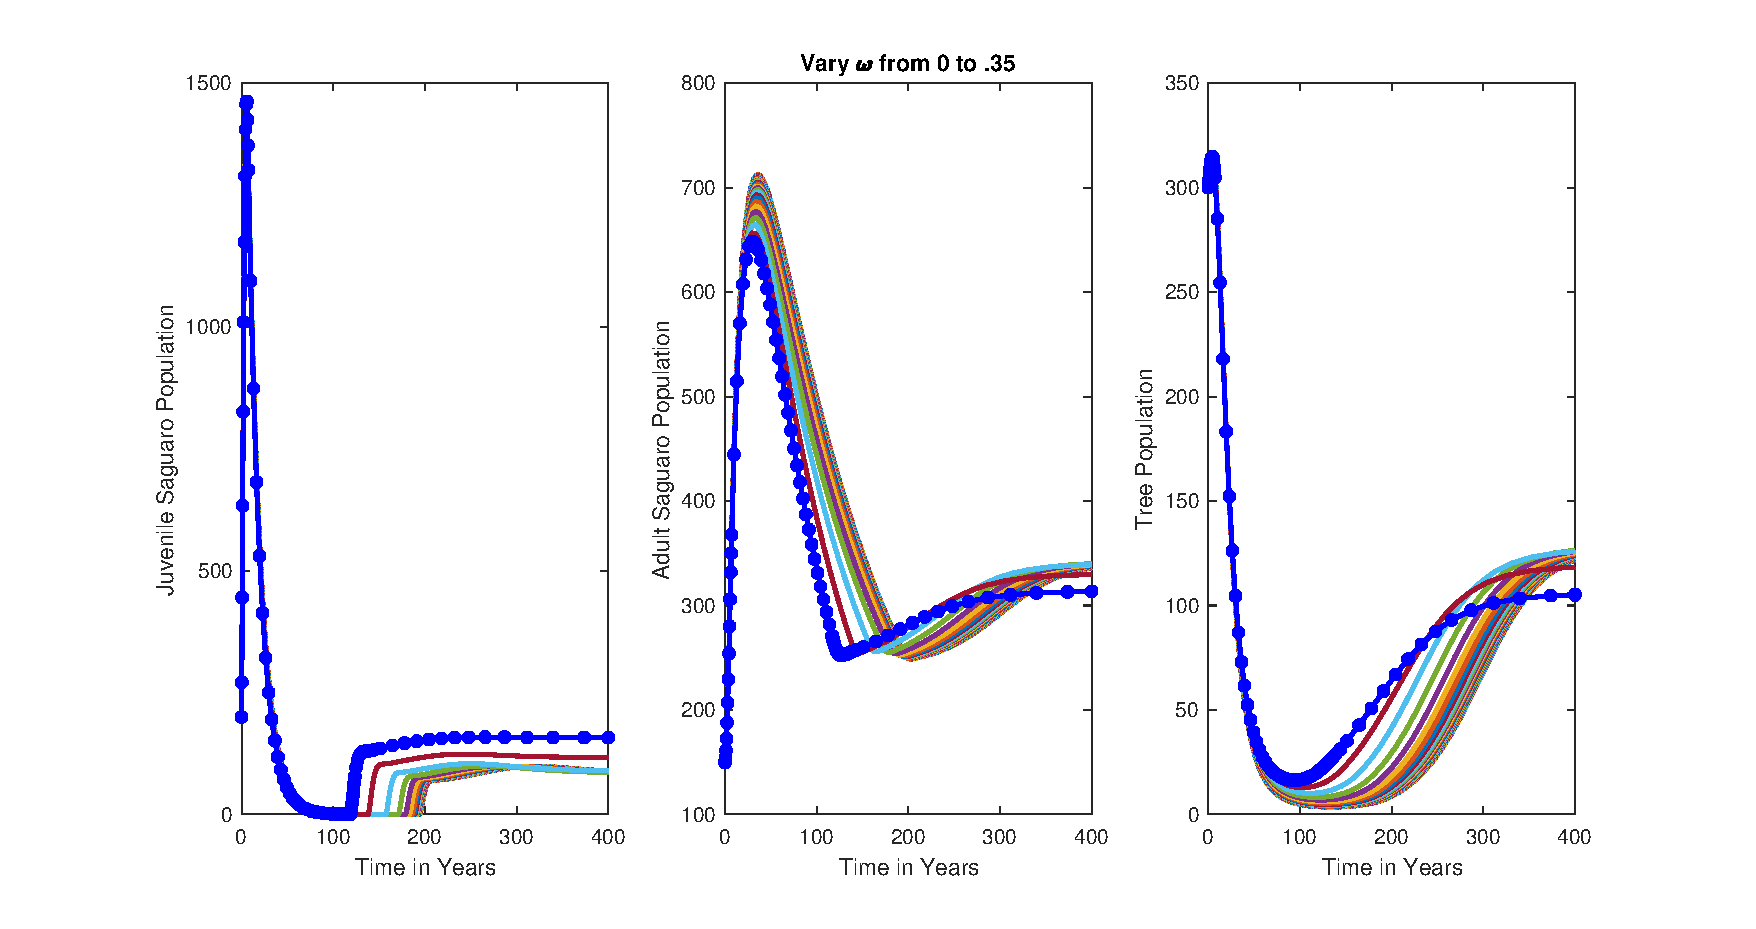
\includegraphics[scale = 0.4]{VaryOmegaWbuffel.eps}
\end{figure}
\begin{figure}
\centering
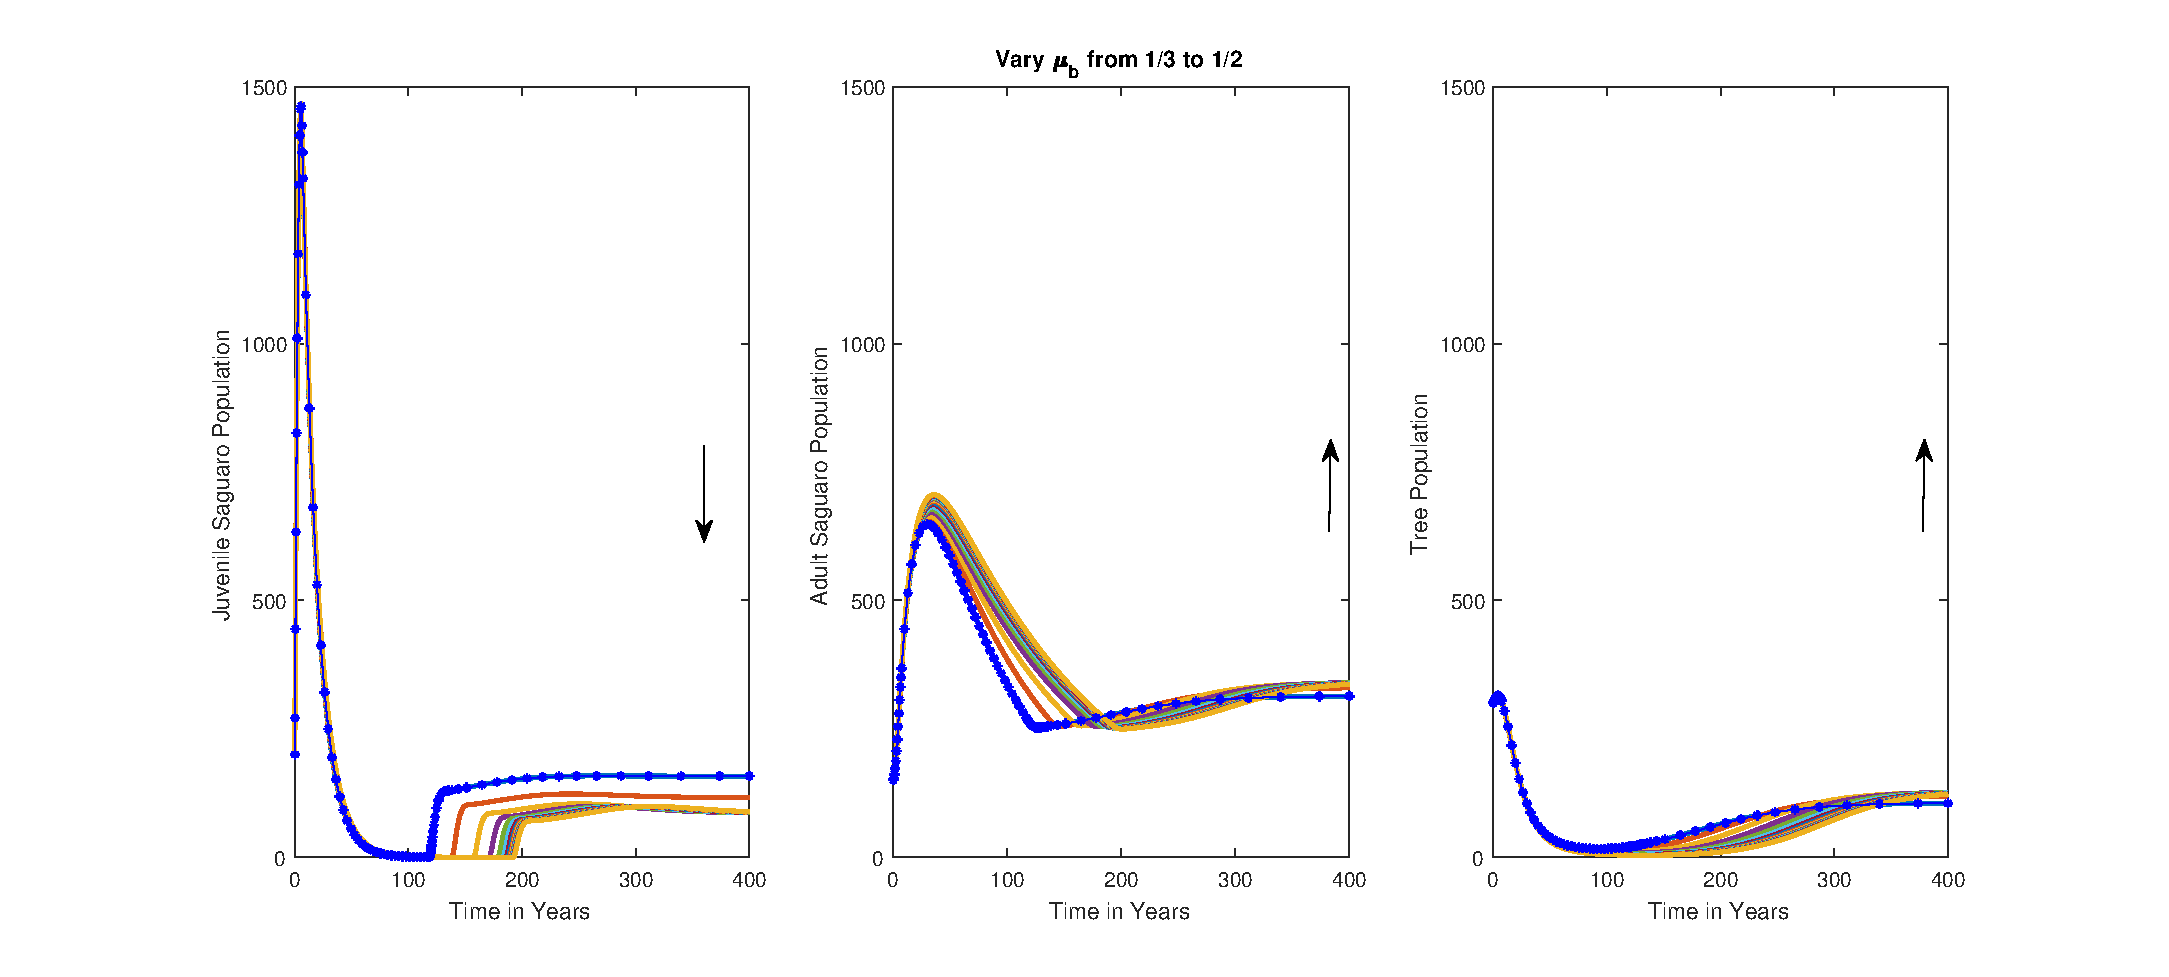
\includegraphics[scale = 0.4]{VaryMubWbuffel.eps}
\tiny{\caption{Decreasing $\omega$, the buffelgrass growth rate, and increasing the $\mu_B$, the harvesting rate of buffelgrass, is shown to increase adult saguaro and nurse tree populations at equilibrium.}}
\end{figure}
\vspace{-4cm}
\section{Local Sensitivity Analysis}
Local sensitivity analysis quantifies the effects of slightly perturbing the value of a critical parameter on a quantity on interest. In this case the value of the critical parameter is changed by one percent change and the quantities of interest are the equilibrium populations. The sign of each sensitivity index gives the direction of the change in the quantity of interest, and the value gives the magnitude of the change in percentage. Sensitivity analyzed without the inclusion of buffelgrass gives the growth rate of trees, $\phi$ as the most sensitive parameter. This means planting more trees will increase both the nurse tree and saguaro populations.\\

\vspace{-2cm}
\begin{table}
\small{
\begin{center}
\hspace{-.8cm}
\begin{tabular}{|c|c|c|c|c|}\hline
{Sensitivity Analysis}
& $r$ & $b$ & $\phi$\\
\hline
$S_j$ &  0.0013& 0.1006 & 0.6534\\
\hline
$S_a$ & 0.0013 & 0.1006 & 0.6534\\
\hline
$T$ & -0.0084 & -0.6534 & 2.2520\\
\hline
\end{tabular}
\end{center}
}
\end{table}

Sensitivity analysis after the inclusion of buffelgrass shows that the equilibrium populations are most sensitive to the growth rate, $\omega$, and harvesting rate of buffelgrass, $\mu_B$.\\

\vspace{-1cm}
\begin{table}
\centering
\small{
\begin{center}
\hspace{-.8cm}
\begin{tabular}{|p{2.8cm}|c|c|c|c|c|}\hline
{Sensitivity Analysis}& $\theta_j$ & $\theta_a$ & $\theta_T$ & $\mu_b$ & $\omega$ \\
\hline
$S_j$ &  \num{-3.92e-04} & 0.4916 & -0.0753 & -8.3189 & 8.3232 \\
\hline
$S_a$ & \num{-3.92e-04} & -0.0111 & -0.0753 & 1.7351
 & -1.7354 \\
\hline
$T$ & 0.0028 & 0.0803 & -0.2980 & 4.2973 & -4.2973\\
\hline
$B$ & N/A & N/A & N/A & -20 & 20\\
\hline
\end{tabular}
 \end{center}
  }
\end{table}

\vspace{-1cm}
\section{Conclusions}
The numerical simulations showed that with and without the inclusion of buffelgrass, the saguaro and nurse tree populations are able to coexist. In the absence of buffelgrass, the most efficient way to influence the production of more adult saguaros is to increase the growth rate of trees.Although with the natural wildfire frequency the saguaro and nurse tree populations are able to coexist with buffelgrass, if the wildfire frequency increases, saguaros and nurse trees would be put at risk. The best way to reduce this risk was found to be reducing the buffelgrass population by decreasing the growth rate of the buffelgrass population through herbicide spraying, and increasing the harvesting rate of buffelgrass population through manual pulling.

\end{multicols}

\section{Acknowledgements:}

\small{
We would like to thank the Mathematical and Theoretical Biology Institute (MTBI) co-Directors Dr. Carlos Castillo-Chavez, and Dr. Anuj Mubayi for giving us the opportunity to participate in this research program. We would also like to thank associate director Sherry Woodley, coordinator Ciera Duran and management intern Sabrina Avila for their efforts in providing logistics for activities during MTBI. We also want to give special thanks to Karen Ríos-Soto, Christopher Kribs, Fan Yu, Juan Melendez-Alvarez, Leon M Arriola, and Anuj Mubayi for their contributions throughout this project. The research has been carried at the MTBI which is a Research Experience for Undergraduate (REU) summer program at the Simon A. Levin Mathematical, Computational and Modeling Sciences Center (SAL MCMSC) at Arizona State University (ASU). This project has been partially supported by grants from the National Science Foundation (DMS1263374), the National Security Agency (H98230-15-1-0021), the Office of the President of ASU, and the Office of the Provost at ASU.
}
\end{document}


